\documentclass{article}

\usepackage{../parm}
\begin{document}

    \section{Décodeur 7 segment}

    \subsection{Introduction}

    Nous allons commencer par une prise en main de \texttt{Logisim} en réalisant un décodeur 7 segments.
    Ce type d'afficheur est un grand classique en ce qui concerne l'affichage de caractères hexadécimaux.

    Le principe de cet afficheur est très simple, En allumant plusieurs segments en même temps nous allons pouvoir représenter les caractères suivants :
    0,1,2,3,4,5,6,7,8,9,A,B,C,D,E,F.

    \begin{figure}[H]
        \makebox[\textwidth]{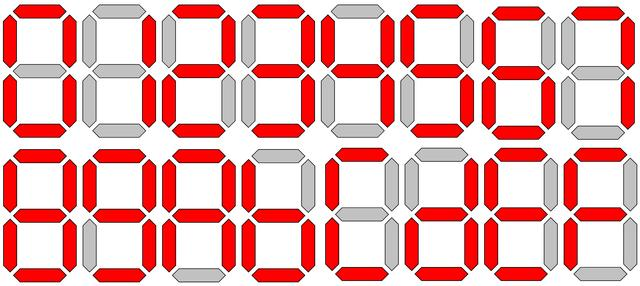
\includegraphics[width=15cm]{pictures/7seg.jpg}}
        \caption{Un affichage hexadécimal par 7 segments. Merci à \href{https://twitter.com/skywodd}{@Skywodd} - \url{https://www.carnetdumaker.net/}}
    \end{figure}

    L'objectif est ici est de recevoir une information sur 4 bits (comprise entre \texttt{0b0000} et \texttt{0b1111}) et de la traduire sur 7 bits correspondant aux segments à allumer et à ceux à éteindre\footnote{\url{http://www.electronics-tutorials.ws/blog/7-segment-display-tutorial.html}}.

    \subsection{Table de correspondance}
    Nous allons ici associer à chaque valeur à sa décomposition en segment d'après le schéma suivant :
    \begin{figure}[H]
        \makebox[\textwidth]{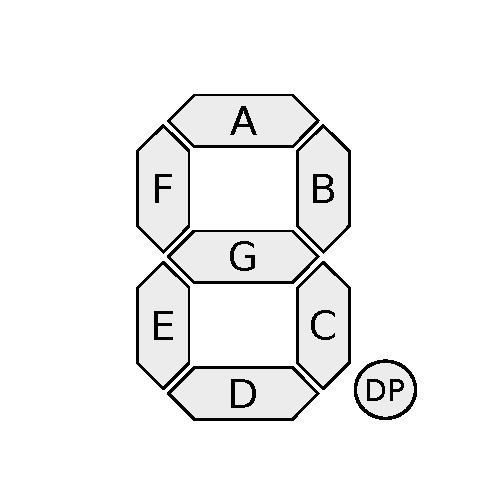
\includegraphics[height=3cm]{pictures/7segdetails.pdf}}
        \caption{Détail et Annotation d'un 7 segment par \href{https://commons.wikimedia.org/wiki/User:H2g2bob}{H2g2bob} - \ccLogo\ccAttribution\ccShareAlike}
    \end{figure}

    \begin{table}[H]
        \centering
        \begin{tabular}{|c|c|c|c|c|c|c|c|}
            \hline
            & \multicolumn{7}{c|}{Individual Segments} \\
            \hline
            Display & A & B & C & D & E & F & G \\
            \hline
            0       & 1 & 1 & 1 & 1 & 1 & 1 & 0 \\
            \hline
            1       & 0 & 1 & 1 & 0 & 0 & 0 & 0 \\
            \hline
            2       & 1 & 1 & 0 & 1 & 1 & 0 & 1 \\
            \hline
            3       & 1 & 1 & 1 & 1 & 0 & 0 & 1 \\
            \hline
            4       & 0 & 1 & 1 & 0 & 0 & 1 & 1 \\
            \hline
            5       & 1 & 0 & 1 & 1 & 0 & 1 & 1 \\
            \hline
            6       & 1 & 0 & 1 & 1 & 1 & 1 & 1 \\
            \hline
            7       & 1 & 1 & 1 & 0 & 0 & 0 & 0 \\
            \hline
            8       & 1 & 1 & 1 & 1 & 1 & 1 & 1 \\
            \hline
            9       & 1 & 1 & 1 & 1 & 0 & 1 & 1 \\
            \hline
            A       & 1 & 1 & 1 & 0 & 1 & 1 & 1 \\
            \hline
            B       & 0 & 0 & 1 & 1 & 1 & 1 & 1 \\
            \hline
            C       & 1 & 0 & 0 & 1 & 1 & 1 & 0 \\
            \hline
            D       & 0 & 1 & 1 & 1 & 1 & 0 & 1 \\
            \hline
            E       & 1 & 0 & 0 & 1 & 1 & 1 & 1 \\
            \hline
            F       & 1 & 0 & 0 & 0 & 1 & 1 & 1 \\
            \hline
        \end{tabular}
        \caption{Décomposition des caractères hexadécimaux en segments}
    \end{table}

    \subsection{Mise en place sur logisim}

    La table de vérité présentée dans la section précédente peut être utilisée pour obtenir une fonction simplifiée de chaque segment en utilisant les tables de Karnaugh\footnote{\url{https://fr.wikipedia.org/wiki/Table_de_Karnaugh}}.
    \texttt{Logisim} embarque une fonctionnalité permettant d'effectuer cette analyse de manière simplifiée.
    Pour cela il est nécessaire de lancer \texttt{Logisim} avec l'option -analyze, soit dans notre cas :

    \begin{lstlisting}[language=bash]
java -Dsun.java2d.opengl=true -jar logisim-evolution.jar -analyze
    \end{lstlisting}

    En utilisant ce paramètre une option apparaît dans le menu "Projet"->"Analyser le circuit".
    Il est possible dans l'onglet "table" de remplir la table de vérité du circuit.
    Une fois le tableau complété, cliquer sur "Construire le circuit" générera le circuit correspondant.
    Ce dernier devrait ressembler à ceci :
    \begin{figure}[H]
        \makebox[\textwidth]{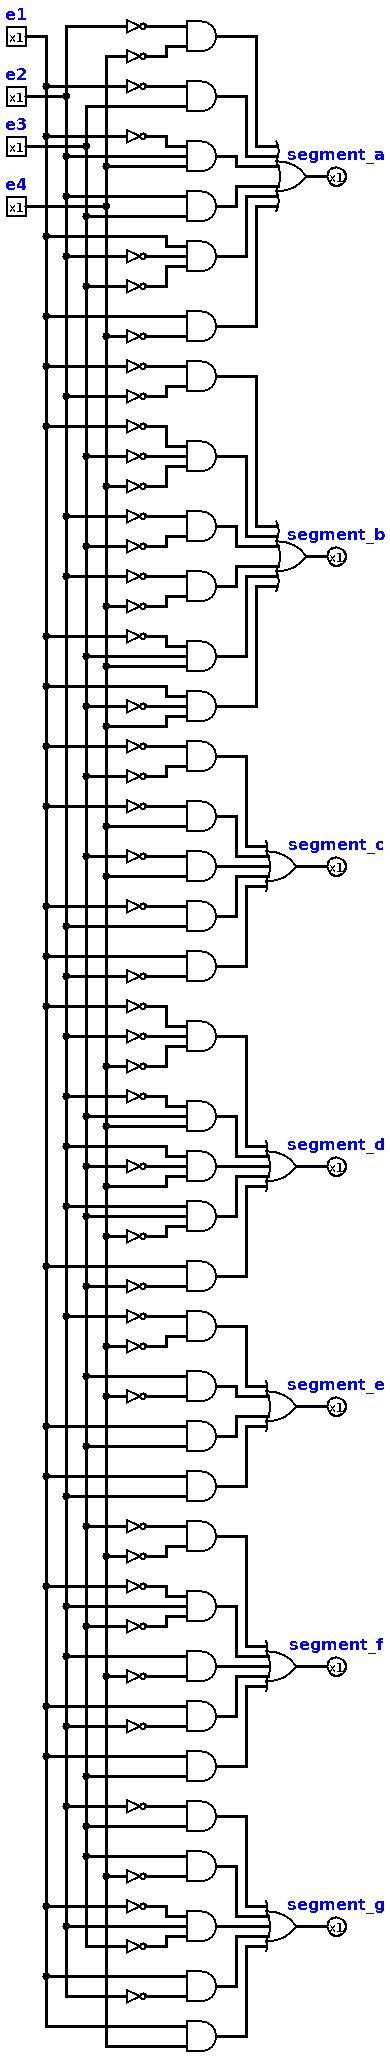
\includegraphics[width=4cm]{pictures/sevendecoder.png}}
        \caption{Contenu du composant "Seven segment decoder"}
    \end{figure}


\end{document}